\documentclass[14pt]{beamer}

\usetheme{Madrid}

% Add frame numbers
\setbeamertemplate{page number in head/foot}[framenumber]

\usepackage{amsmath, amssymb}
\usepackage{tikz}

\newcommand{\CMA}{Causal Mediation Analysis}
\newcommand{\bE}{\mathbb{E}}
\newcommand{\GLMMs}{Generalized Linear Mixed Models}

\title[]{Statistical Considerations in Multilevel Mediation Analysis}
\author{William Ruth}
\institute[]{Collaborators: Rado Ramasy, Rowin Alfaro, Ariel Mundo, Bouchra Nasri}
\date{\vspace{-3cm}}
\titlegraphic{\includegraphics[width=2cm]{Logos/CANSSI_Logo.png} \hspace{2cm} \includegraphics[width=4cm]{Logos/Logo_UdeM-CMJN.jpg}}


\begin{document}

\begin{frame}
    \titlepage
\end{frame}

\begin{frame}{Outline}
    \begin{itemize}
        \setlength{\itemsep}{1em}
        \item The Problem
        \item Causal Mediation Analysis
        \item Generalized Linear Mixed Models
        \item The Bootstrap
    \end{itemize}
\end{frame}

\begin{frame}{Example}
    \begin{itemize}
        \item Goal: Understand adherence to restrictive measures
        \begin{itemize}
            \item E.g. Lockdowns
            \item Both past and future \newline
        \end{itemize}
        \item Influence of news source
        \begin{itemize}
            \item How trustworthy? \newline
        \end{itemize}
        \item Disentangle influence on future from influence on past
    \end{itemize}
    
\end{frame}


\begin{frame}{Example}
        \begin{figure}[H]
            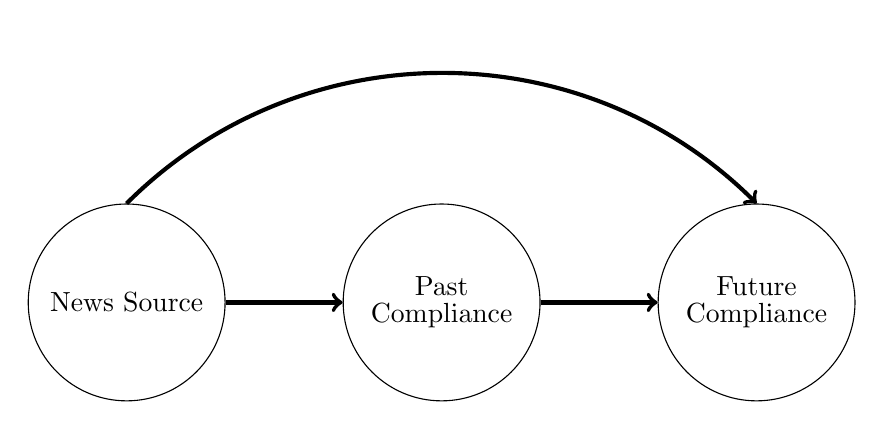
\begin{tikzpicture}
                % Circles with labels
                \node at (0,0) [circle, draw, minimum size=2.5cm] (news) {News Source};
                \node at (4,0) [circle, draw, minimum size=2.5cm] (past) {\shortstack{Past\\Compliance}};
                \node at (8,0) [circle, draw, minimum size=2.5cm] (future) {\shortstack{Future\\Compliance}};
                
                % Arrows
                \draw[->, line width=1.5pt] (news.east) -- (past.west);
                \draw[->, line width=1.5pt] (past.east) -- (future.west);
                \draw[->, line width=1.5pt, bend left] (news.north) to [out=45,in=135] (future.north); 
                
                \end{tikzpicture}
    \end{figure}
\end{frame}

\begin{frame}{Example}
    Terminology
    \begin{columns}
        \column{0.6\textwidth}
        \begin{itemize}
            \item Top path: {Direct effect}
            \item Center path: {Indirect effect}
            \item Combined: {Total effect}
        \end{itemize}
        \column{0.4\textwidth}
        \begin{itemize}
            \item Exposure: $X$
            \item Outcome: $Y$
            \item Mediator: $M$
        \end{itemize}
    \end{columns}
    
\end{frame}




\begin{frame}{Mediation Analysis}
    \begin{figure}[H]
        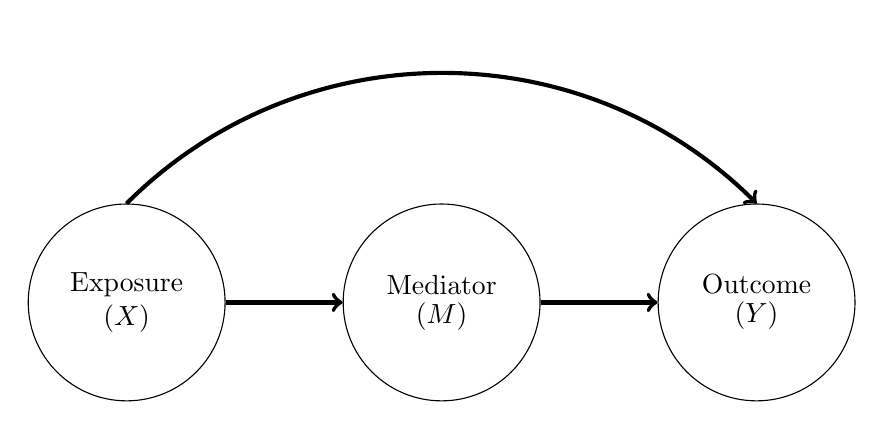
\begin{tikzpicture}
            % Circles with labels
            \node at (0,0) [circle, draw, minimum size=2.5cm] (X) {\shortstack{Exposure\\($X$)}};
            \node at (4,0) [circle, draw, minimum size=2.5cm] (M) {\shortstack{Mediator\\($M$)}};
            \node at (8,0) [circle, draw, minimum size=2.5cm] (Y) {\shortstack{Outcome\\($Y$)}};
            
            % Arrows
            \draw[->, line width=1.5pt] (X.east) -- (M.west);
            \draw[->, line width=1.5pt] (M.east) -- (Y.west);
            \draw[->, line width=1.5pt, bend left] (X.north) to [out=45,in=135] (Y.north); 
            
            \end{tikzpicture}
    \end{figure}
\end{frame}

\begin{frame}{Mediation Analysis}
    Separate \textbf{Total Effect} of $X$ on $Y$ into
    \begin{itemize}
        \item \textbf{Direct Effect}
        \item \textbf{Indirect Effect}\newline
    \end{itemize}

    Traditionally, use regression
\end{frame}

\begin{frame}{Mediation Analysis}
    Continuous outcome and mediator:
    \begin{itemize}
        \item $Y = \alpha_0 + \alpha_1 M + \alpha_2 X + \varepsilon_Y$
        \item $M = \beta_0 + \beta_1 X + \varepsilon_M$ \newline
    \end{itemize}

    
    \textbf{Direct Effect}: $\alpha_2$
    \begin{itemize}
        \item ``$X$ in $Y$''
    \end{itemize}
    \textbf{Indirect Effect}: $\alpha_1 \cdot \beta_1$
    \begin{itemize}
        \item ``$M$ in $Y$'' $\cdot$ ``$X$ in $M$''
    \end{itemize}
    \textbf{Total Effect}: $\alpha_2 + \alpha_1 \cdot \beta_1$

\end{frame}

\begin{frame}{Mediation Analysis}
    Popular approach
    \begin{itemize}
        \item A bit outdated\ldots \newline
    \end{itemize}

    More popular: Causal mediation analysis
    
\end{frame}

\begin{frame}{Causal Mediation Analysis}
    Assume that $X$ \textit{causes} $Y$\newline

    Counterfactuals:
    \begin{itemize}
        \item What value would $Y$ take if $X$ were set to a particular level?
        \item Write $Y_x$ for the value of $Y$ when $X=x$
        \item If $X\neq x$ then $Y_x$ is literally a ``counterfactual'' 
    \end{itemize}
\end{frame}

\begin{frame}{Causal Mediation Analysis}
    Example:
    \begin{itemize}
        \item Alice only reads scientific publications and will follow all lockdown mandates
        \item What if she instead only read Facebook?\newline
        \item $Y_{Science}(Alice) = \mathrm{follow}$
        \item $Y_{Facebook}(Alice) = \mathrm{follow}$
    \end{itemize}
\end{frame}

\begin{frame}{Causal Mediation Analysis}
    Example:
    \begin{itemize}
        \item Bob also only reads scientific publications and will follow all lockdown mandates, but is more susceptible to being influenced \newline
        \item $Y_{Science}(Bob) = \mathrm{follow}$
        \item $Y_{Facebook}(Bob) = \mathrm{not\ follow}$
    \end{itemize}
\end{frame}

\begin{frame}{Causal Mediation Analysis}
    \begin{itemize}
        \item We only observe one outcome per individual\newline

        \item Explore population-level effects by averaging\newline

        \item Define mediation effects in terms of expected counterfactuals
    \end{itemize}
\end{frame}

\begin{frame}{Causal Mediation Analysis}
    \textbf{Total Effect}: $\mathbb{E}(Y_{x'} - Y_{x})$
    \begin{itemize}
        \item Effect on outcome when we change exposure from $X=x$ to $X=x'$ \newline
    \end{itemize}

    Other effects involve dependence on the mediator:
    \begin{itemize}
        \item $Y_{xm}$: Value of outcome when
        \begin{itemize}
            \item Exposure ($X$) is set to $x$
            \item Mediator ($M$) is set to $m$
        \end{itemize}
        \item $M_x$: Value of mediator when
        \begin{itemize}
            \item Exposure ($X$) is set to $x$
        \end{itemize}
        \item Can combine these: $Y_{x M_x}$ or $Y_{x M_{x'}}$
    \end{itemize}

\end{frame}

\begin{frame}{Causal Mediation Analysis}
    \textbf{Controlled Direct Effect}: $\mathbb{E}(Y_{x'm} - Y_{xm})$
    \begin{itemize}
        \item Effect of changing exposure with mediator held fixed \newline
    \end{itemize}

    \textbf{Natural Direct Effect}: $\mathbb{E}(Y_{x'M_{x}} - Y_{xM_{x}})$
    \begin{itemize}
        \item Effect of changing exposure when we don't interfere with the mediator  \newline
    \end{itemize}

    \textbf{Natural Indirect Effect}: $\mathbb{E}(Y_{xM_{x'}} - Y_{xM_{x}})$
    \begin{itemize}
        \item Effect of changing which exposure value is seen by the mediator while holding fixed which exposure value is seen by the outcome
    \end{itemize}
\end{frame}

\begin{frame}{\CMA}
    In our example
    \begin{itemize}
        \item Controlled Direct Effect: Effect of increasing news trustworthiness if the whole population followed guidelines in the past
        \item Natural Direct Effect: Effect of increasing news trustworthiness independent of any possible increase in past compliance
        \item Natural Indirect Effect: Effect of increasing past compliance if everyone only got news from Facebook
    \end{itemize}
\end{frame}

\begin{frame}{\CMA}
    How does causality change our analysis? \newline

    Still fit regression models, but include interaction terms between exposure and mediator
    \begin{itemize}
        \item $Y = \alpha_0 + \alpha_1 M + \alpha_2 X + \alpha_3 M \cdot X + \varepsilon_Y$
        \item $M = \beta_0 + \beta_1 X + \varepsilon_M$ \newline
    \end{itemize}

    Direct and indirect effects now depend on the levels of the exposure

\end{frame}


\begin{frame}{\CMA}
    Discussion so far has involved continuous mediator and outcome
    \begin{itemize}
        \item What about binary or categorical \newline
    \end{itemize}

    Individuals might also be clustered
    \begin{itemize}
        \item E.g. Within countries
    \end{itemize}

\end{frame}

\begin{frame}{\CMA}
    Binary variables is pretty straightforward
    \begin{itemize}
        \item Instead of linear regression, use logistic regression
        \item Re-define mediation effects as odds-ratios of counterfactual probabilities
        \item Formulas relating mediation effects to regression coefficients change \newline
    \end{itemize}

    Extend to more than 2 categories using binary indicators
\end{frame}

\begin{frame}{\CMA}
    Clustered data more complicated \newline

    Standard approach is multi-level modelling
    \begin{itemize}
        \item I.e. Add random effects which vary across clusters \newline
    \end{itemize}

    Combined with categorical variables: 
    \begin{itemize}
        \item Generalized linear mixed models (GLMMs)
    \end{itemize}
\end{frame}


\begin{frame}{Generalized Linear Mixed Models}
    The core idea is to augment our set of covariates
    \begin{itemize}
        \item Coefficients of these new covariates are random variables which vary across groups/clusters \newline
    \end{itemize}

    In the linear setting:
    \begin{itemize}
        \item Old model: $Y = \alpha_0 + \alpha_1 X_1 + \ldots + \alpha_p X_p + \varepsilon$
        \item New model: $Y = \alpha_0 + \alpha_1 X_1 + \ldots + \alpha_p X_p + \mathbf{u_1 Z_1 + \ldots + u_q Z_q} + \varepsilon$ \newline
    \end{itemize}

    


\end{frame}

\begin{frame}{\GLMMs}
    The $Z$'s are fixed, known covariates
    The $u$'s are random variables
    \begin{itemize}
        \item I.e. Random effects \newline
    \end{itemize}

    It's possible for the $X$'s and $Z$'s to overlap
    \begin{itemize}
        \item The coefficient on such a covariate has the form $\alpha_j + u_{k}$
        \item I.e. Mixed effect
    \end{itemize}

\end{frame}


\begin{frame}{\GLMMs}
    Extend to generalized linear models in the usual way \newline

    Choose response distribution and link function as for ordinary GLMs \newline

    Linear predictor now has a random effects component \newline
\end{frame}

\begin{frame}{\GLMMs}
    Why bother?
    \begin{itemize}
        \item E.g. Measured some but not all levels of a categorical variable
        \item Estimate covariance matrix of random effects
        \item Test for non-zero variance of each random effect \newline
    \end{itemize}

    ``Predict'' level of random effects for each group
    \begin{itemize}
        \item Our main focus
        \item Conditional mean or conditional mode of random effects given response
    \end{itemize}
\end{frame}

\begin{frame}{\GLMMs}
    In our example:
    \begin{itemize}
        \item Data collected from 11 different countries
        \item Predict country-specific random effects
        \item Use country-specific coefficients in formulas for mediation effects
        \item Test for significant mediation effects within each country \newline
    \end{itemize}

    Uncertainty quantification for predicted random effects is challenging
\end{frame}

\begin{frame}{The Bootstrap}
    Goal is to circumvent analytical calculation of standard errors \newline

    Replace hard math with hard computing
    \begin{itemize}
        \item Thank you DRAC
    \end{itemize}

    
\end{frame}

\begin{frame}{The Bootstrap}
    Core idea:
    \begin{itemize}
        \item Standard error (SE) is standard deviation from sampling distribution
        \item If we could draw more samples, we could directly estimate SE
        \item We can't sample from the population, but we can estimate the population distribution
        \item Sample from estimated population distribution
        \item Use approximate samples to compute approximate SE
    \end{itemize}
\end{frame}

\begin{frame}{The Bootstrap}
    Different ways to estimate population distribution
    \begin{itemize}
        \item Non-parametric
        \item Parametric \newline
    \end{itemize}

    Sampling and computing statistic of interest many times can be computationally challenging
    \begin{itemize}
        \item Embarrassingly parallelizable \newline
    \end{itemize}

    Different ways to construct confidence intervals
    \begin{itemize}
        \item Percentile, Basic, Wald
    \end{itemize}
\end{frame}




\begin{frame}{The Bootstrap}
    Non-parametric distribution estimation
    \begin{itemize}
        \item Simplest way to estimate a distribution
        \item Put equal weight on each observation, zero weight everywhere else
        \item Simulation consists of sampling from observed data with replacement \newline
    \end{itemize}

    Parametric distribution estimation
    \begin{itemize}
        \item Use estimated parameter values in assumed model
        \item Simulate directly 
    \end{itemize}

\end{frame}

\begin{frame}{The Bootstrap}
    Non-parametric bootstrap in our problem
    \begin{itemize}
        \item Sample with replacement separately within each country
    \end{itemize}
    
    Parametric bootstrap in our problem is more involved
    \begin{enumerate}
        \item Generate random effects for both outcome and mediator models
        \item Calculate linear predictor for mediator
        \item Simulate mediator
        \item Calculate linear predictor for outcome
        \item Simulate outcome
        \item Repeat for each country
    \end{enumerate}
    
\end{frame}

\begin{frame}{The Bootstrap}
    Repeat the algorithm many times to get a bunch of samples \newline
 
    Estimate mediation effects for each sample 
    \begin{itemize}
        \item Gives a distribution for each mediation effect \newline
    \end{itemize}

    Compare these ``bootstrap distributions'' with mediation effects from our original dataset
    \begin{itemize}
        \item Construct confidence intervals for true mediation effects
        \item Many alternatives
    \end{itemize}
\end{frame}


\begin{frame}{The Bootstrap}
    Percentile confidence interval
    \begin{itemize}
        \item $95\%$ interval is the middle $95\%$ of the bootstrap distribution \newline
    \end{itemize}

    Basic confidence interval
    \begin{itemize}
        \item Twice estimate from original dataset minus endpoints of percentile interval \newline
    \end{itemize}

    Wald confidence interval
    \begin{itemize}
        \item Estimate from original dataset $\pm 1.96$ times standard deviation of bootstrap distribution
    \end{itemize}
\end{frame}

\begin{frame}{The Bootstrap}
    Many other methods exist as well, e.g.,
    \begin{itemize}
        \item Studentized interval
        \item Bias-corrected interval
        \item Bias-corrected and accelerated interval \newline
    \end{itemize}

    Choosing which to use is, in general, a hard problem
\end{frame}

\begin{frame}{Putting it All Together}
    Define direct, indirect and total effects using counterfactuals \newline

    Estimate these effects across countries using generalized linear mixed models \newline

    Construct confidence intervals for estimated effects using the bootstrap
\end{frame}

\begin{frame}{Acknowledgements}
    Collaborators:
    \begin{itemize}
        \item Rado Ramasy
        \item Rowin Alfaro
        \item Ariel Mundo
        \item Bouchra Nasri \newline
    \end{itemize}

    Funding:
    \begin{itemize}
        \item Canadian Statistical Sciences Institute
    \end{itemize}
\end{frame}

\begin{frame}
    \centering
    \Huge Thank You
\end{frame}

\end{document}
